\chapter{Result and Discussions}
\label{results}
Once all software packages are aligned under a single python script, the python script is fired into the HPC cluster. After covering a considerable amount of time, the results are extracted, and the post-processing is carried using Paraview. This chapter contains detailed information about the number of computational hours used, the CFD solver setup, optimized wings, and more importantly, the comments over the obtained results.

The objective function that is aimed is the drag coefficient minimization. Furthermore, the drag is made up of two parts. They are pressure drag and the induced drag. Since this work involves the inviscid solution, the drag represented here will be the induced drag alone. Equation \ref{induced_drag} represents the equation for induced drag evaluation \cite{Poole1}. 
\begin{equation}
C_{D_{i}}=\frac{C_{L}^{2}}{\pi A R}(1+\delta)
\label{induced_drag}
\end{equation}
where,\\
$$\delta=8\left(\frac{3 \pi}{2} \frac{C_{M_{x}}}{C_{L}}-1\right)^{2}$$

For the given problem (ADODG case 6) with aspect ratio 6, the theoretical minimum induced drag is found to be 25.5 counts (1 count = $10^{-3}$ drag units).

\section{Algorithm Assessment: Finding local minima for the test functions.}
The niching algorithm is initially tested on an analytical test function to assess their performance. Appendix \ref{app_c} contains the test functions that are analyzed. For example, consider the sphere function, as shown in equation \ref{Sphere function}.

\begin{equation}
f(\mathbf{x})=\sum_{i=1}^{d} x_{i}^{2}
\label{sphere_function}
\end{equation}

Further, the test function is subjected to constraints as mentioned in \cite{Poole3}. There exists four optima located at (1, 1), (-1, 1), (-1, -1), and (1, -1). Niching algorithm as mentioned in chapter \ref{niching} are implemented over this test function and the result are promising. Figure \ref{init_pop} illustrates the outcome of fINRAND1 niching algorithm over the given 2-D test function. 
\begin{figure}[!htbp]
\parbox{0.47\linewidth}
    {
    \centering
    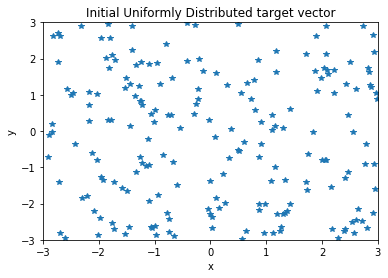
\includegraphics[scale = 0.5]{figures/initial_pop.png}
    \caption{Initial 200 population.}
    \label{init_pop}
    }
\parbox{0.47\linewidth}
    {
    \centering
    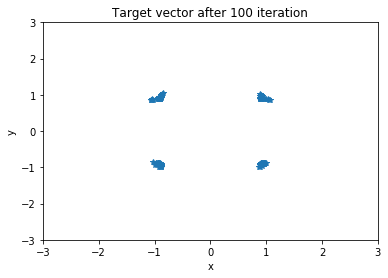
\includegraphics[scale = 0.5]{figures/final_target.png}
    \caption{Optimal points after 100 generations.}
    \label{target_points}
    }
\end{figure}

Overall, a population of 200 are used within the design space $x_1:(3, -3)$ and $x_2:(3, -3)$. A total of 100 generations are carried out to get an optimal solution. However, in the case of CFD simulation running for such higher generations seems impractical. A trade-off is required between the generations and the solutions obtained. This confirms that the algorithm is capable of identifying the local optima in a given design space.

\section{Computational power}
In the initial stage, the niching algorithms were tested in the workstation with Intel Xeon W-2155 @ 3.3 GHz, 20 CPU. However, the assigned workstation would not be sufficient to run the full-fledged optimizer. As a result, the entire work is executed in the HPC cluster containing 56 CPU with Intel Xeon E5-2690 @ 2.6 GHz. This work demands for 20 CPU of a given compute node and takes less than 180 minutes to complete a generation.

\section{Grid sensitivity analysis}
In the entire optimization process, the objective function evaluation (CFD simulation) is a bottleneck. With higher mesh points, more will be the computational cost. So it is very crucial to choose the mesh size, which is feasible for given computational power. A baseline wing with two mesh quality is generated. Table \ref{grid_sensitivity} provide additional details about the mesh quality.

\begin{table}[!htbp]
    \centering
    \begin{tabular}{|c|c|c|}\hline
        \textbf{Mesh quality} & \textbf{Surface mesh} & \textbf{Volume mesh} \\\hline
        Coarse  & 150 $\times$ 100 & 0.11m \\
        Fine  & 300 $\times$ 200 & 0.25m \\\hline
    \end{tabular}
    \caption{Grid sensitivity analysis}
    \label{grid_sensitivity}
\end{table}
The baseline wing with coarse mesh (150 along the chord, 100 along the span) would take less than 50 minutes (workstation) to complete the CFD run, whereas, the fine mesh takes about 120 minutes (workstation). Further, with additional lift coefficient constraint the fine mesh completed the CFD run in 180 minutes (workstation). This implies if the problem is set to run in parallel with each CPU assigned to one of the perturbed wings, after every 180 minutes, one optimization generation get completed. 
\begin{figure}[!htbp]
    \centering
    \framebox{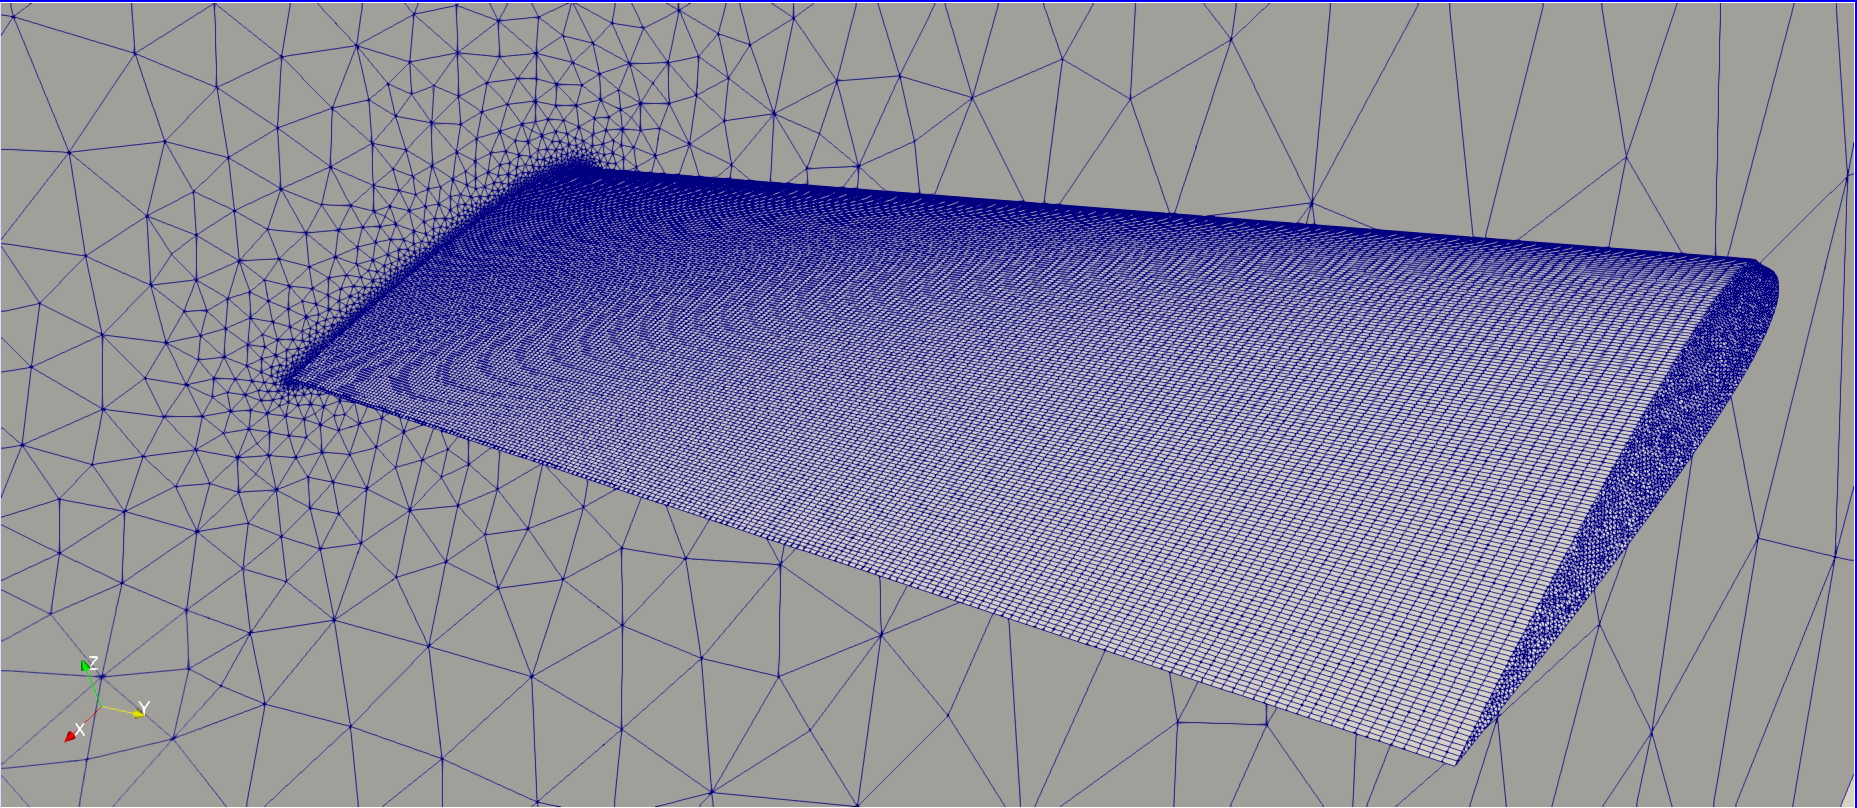
\includegraphics[scale = 0.22]{figures/fine_mesh_wing.png}}
    \caption{Fine mesh with 300 $\times$ 200 surface mesh points.}
    \label{fine_mesh}
\end{figure}

Figure \ref{fine_mesh} represents the fine mesh containing 0.25m mesh points with 300 $\times$ 200 mesh points over the wing surface. The distribution of mesh points at the symmetry surface is appropriate. Cell size is increasing from the wing surface towards the wall surfaces at a rate of 20\%.
\begin{figure}[!htbp]
    \centering
    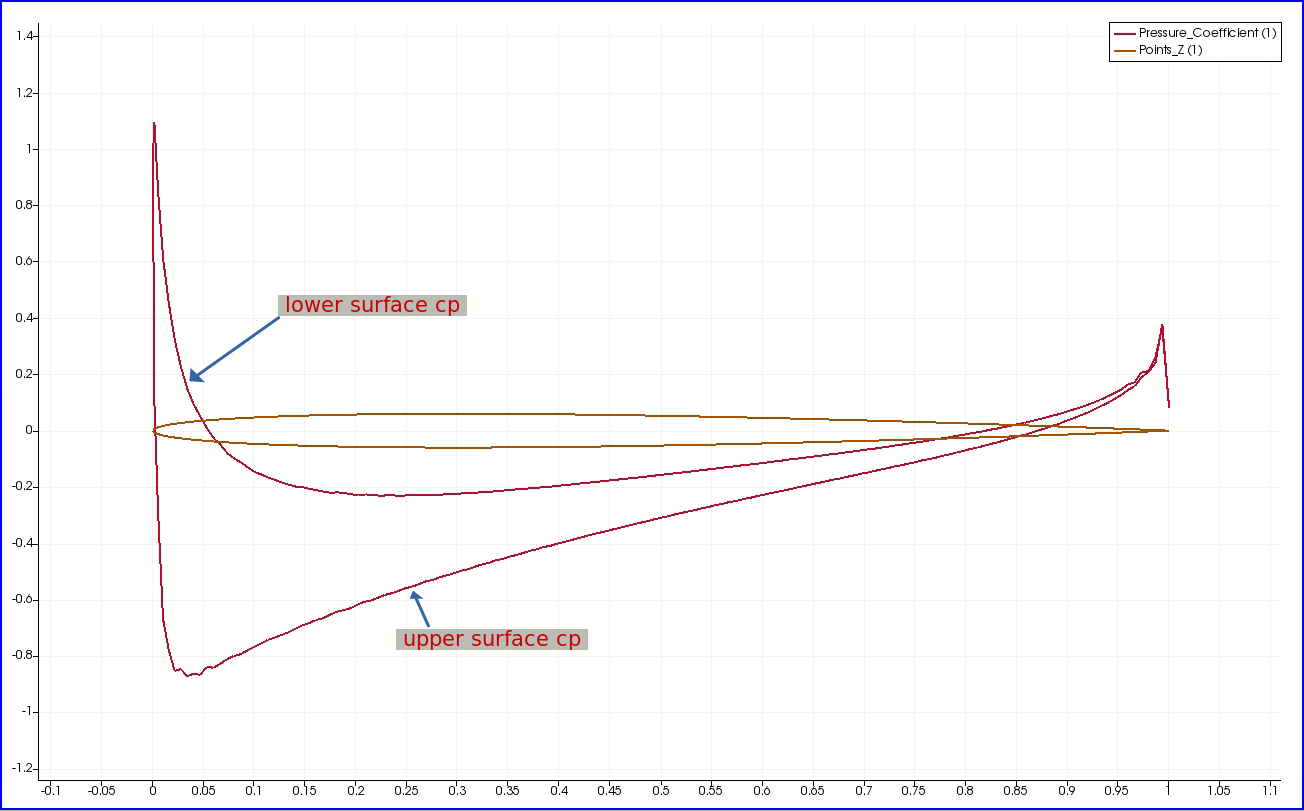
\includegraphics[scale = 0.3]{figures/cp_curve.png}
    \caption{Cp curve at root section of fine mesh (300 $\times$ 200).}
    \label{cp curve}
\end{figure}

Figure \ref{cp curve} represents the coefficient of pressure at the root section of the baseline wing for a fine mesh. The results of the cp curve meet the expected values. There is some disturbance in the Cp curve at the trailing edge. The reason for this is because the airfoil has a sharp trailing edge. The fine mesh appears appropriate to proceed with full optimization.

\section{Multimodality}
In this problem, the flow is subsonic and inviscid. The objective is to minimize the drag coefficient of $C_d$. The Mach number is 0.4. The lift coefficient of $C_l$ is constrained to 0.2625. The angle of attack is varied between -3$^0$ and +6$^0$. The angle of attack is a design variable which is optimized using CFD solver. The root bending moment is constrained to be $\leq$ 0.1039. Geometry is parameterized using the FFD box with 5 points along chord direction, 2 points along the thickness direction, and 6 points along the span direction, resulting in 60 control points. Each perturbed wing can vary in span direction between 2.7 units and 3.3 units. Due to FFD box control points perturbation, the perturbed wing will possess the twist and sweep angles. Each of the control points is perturbed such that it always results in feasible wings. More details on FFD control point perturbation is mentioned in chapter \ref{methodology}.

The first 20 initial geometries (population) generated by the random selection of point within the PCA selected design space is shown in figure \ref{initial_population}. These population cover all the design space like dihedral, taper wings, sweep backward/forward, winglet up/down, and span long/short.

\begin{figure}[!htbp]
    \centering
    \framebox{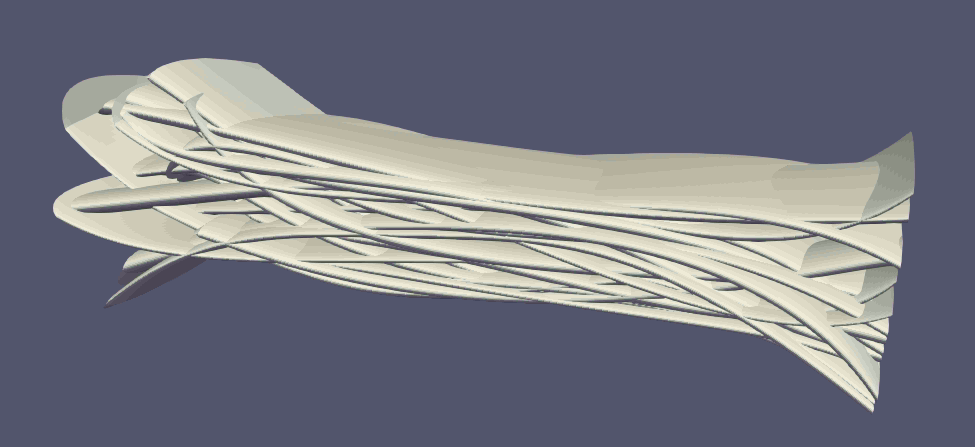
\includegraphics[width=0.95\textwidth, height=70mm]{figures/initial_population.png}}
    \caption{Initial 20 populations.}
    \label{initial_population}
\end{figure}

\begin{figure}[!htbp]
    \centering
    \framebox{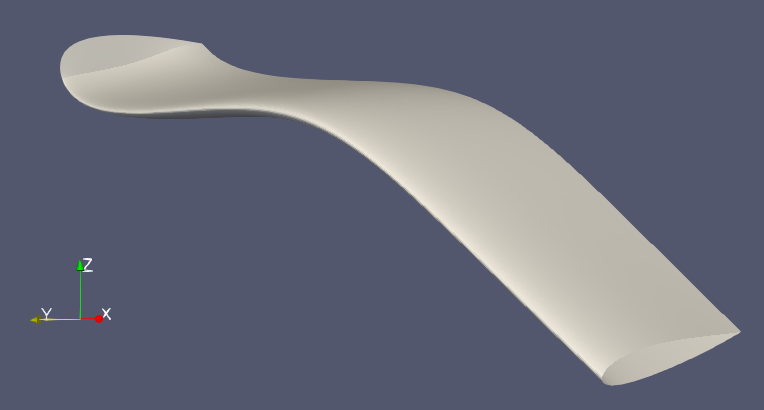
\includegraphics[width=0.95\textwidth, height=70mm]{figures/isoview_localwing_1.png}}
    \caption{Isometric view of local optima 1.}
    \label{isoview_localoptima_1}
\end{figure}

Since the flow is subsonic and inviscid, only the induced drag is present. The baseline (NACA 0012) geometry has $C_d$ of 5.08 $\times$ $10^{-2}$, with $C_l$ constraint satisfied by adjusting the angle of attack. After 1000 objective function evaluation, the first local optima was found to possess the $C_d$ value of 1.12 $\times 10^{-2}$. Figure \ref{isoview_localoptima_1} and \ref{frontview_localoptima_1} illustrates the isometric and leading-edge view of local optima 1 respectively.

\begin{figure}[!htbp]
    \centering
    \framebox{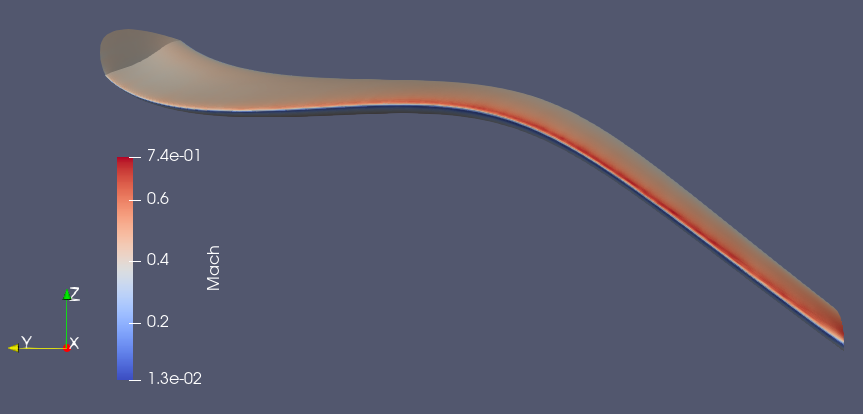
\includegraphics[width=0.95\textwidth, height=70mm]{figures/frontview_localwing_1.png}}
    \caption{Leading edge view of local optima 1.}
    \label{frontview_localoptima_1}
\end{figure}


Figure \ref{cp_curve in span direction} represents the Cp distribution for local optima 1 at three sections, that is, root section, midsection, and tip section. At root section, near the leading edge, there is a sharp decline in Cp value in the upper surface. The reason for this is incorrect volume mesh generation around the leading edge. A similar explanation can be provided for trailing edge Cp disturbance. The airfoil is twisted by small value and lift by a unit in the midsection of the span. At the tip section, the results got disrupted entirely. The airfoil is highly perturbed, resulting in negative lift.

After further analysis, it was found that the glyph script, that was designed to automate the volume mesh generation is incorrect. The script could not generate enough mesh points to get correct CFD results. No conclusion can be drawn from incorrect CFD solution. Due to insufficient time, the glyph script could not be corrected. However, assuming that the CFD results are correct, table \ref{optimal shape} represents local optima with additional details. More on these optima is covered in the upcoming section.

\begin{figure}[!htbp]
  \parbox{0.47\linewidth}{
    \centering
    \framebox{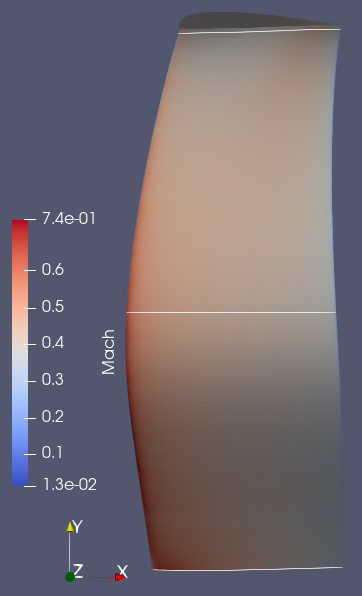
\includegraphics[width=0.9\linewidth, height=150mm]{figures/local_wing_1_span.png}}
    }
  \parbox{0.47\linewidth}{
    \centering
    \framebox{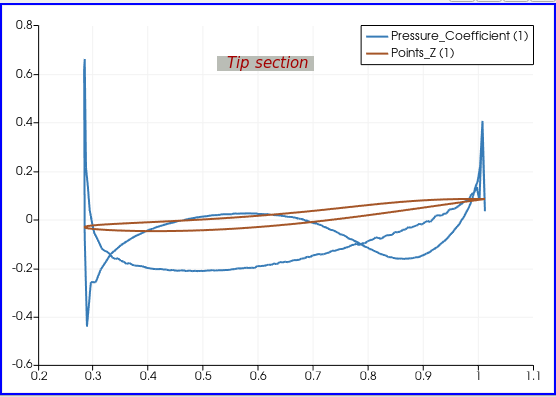
\includegraphics[scale=0.35]{figures/local_wing_1_tip_section.png}}
    \framebox{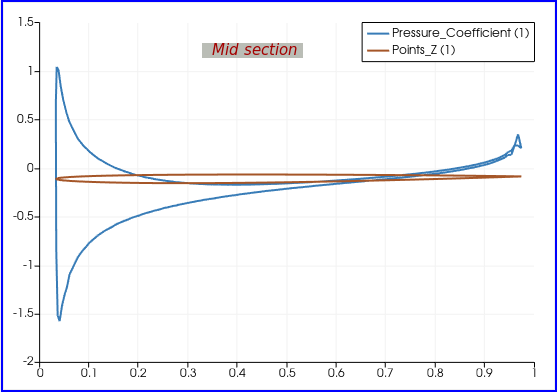
\includegraphics[scale=0.35]{figures/local_wing_1_mid_section.png}}
    \framebox{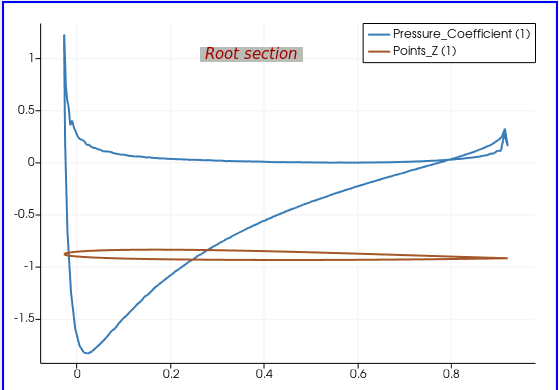
\includegraphics[scale=0.35]{figures/local_wing_1_root_section.png}}
    }
    \caption{Cp distribution at various sections in local optima 1 along span directions.}
    \label{cp_curve in span direction}
\end{figure}

\begin{table}[!htbp]
    \centering
    \begin{tabular}{|c|c|c|c|c|c|c|}\hline
          & $C_l$ & $C_d$ & $C_{M_x}$ & $AoA$ & Span & Obj.diff \\\hline
        local optima 1 & 0.2625 & 0.01120   & 0.1038 & 5.535$^0$ & 2.779 & 0.0\%\\
        local optima 2 & 0.2625 & 0.01203   & 0.1005 & 3.213$^0$ & 2.918 & 7.4\%\\
        local optima 3 & 0.2625 & 0.01204   & 0.1028 & 1.972$^0$ & 2.726 & 7.5\%\\
        local optima 4 & 0.2625 & 0.01215   & 0.998  & 2.774$^0$ & 3.291 & 8.4\%\\ \hline
    \end{tabular}
    \caption{$C_d$ values for various local optima.}
    \label{optimal shape}
\end{table}

\section{Discussion}

After a detailed examination of all steps, it is noticed that the wing parameterization, the FFD box implementation, the PCA implementation, and niching algorithm implementation is working correctly. The sole issue for incorrect results was inadequate volume mesh points. To reduce the computational cost, the number of mesh points is kept on the lower side (0.25m). With the same number of mesh points, the grid sensitivity analysis is carried out for baseline geometry, and the results (cp curve) seems acceptable. 

Following this, the same glyph script, which is meant for volume mesh generation, is used to generate the volume mesh for perturbed wings. However, at the end of full optimization, it was found that the grid resolution and grid clustering algorithm was not adequate, which resulted in erroneous flow-field. Also, at some sections in the optimal wings, inverted airfoils are generated. The cp curve shows inappropriate behaviour at those sections and is propagated through all sections of the given wing. Figure \ref{cp_curve in span direction} depicts the same.

The present work aimed to identify the existence of multimodality in a given design space. However, due to the present situation, COVID-19 pandemic, the work is partially completed. Also, glyph script can not be corrected remotely.

\begin{figure}[!htbp]
    \centering
    \framebox{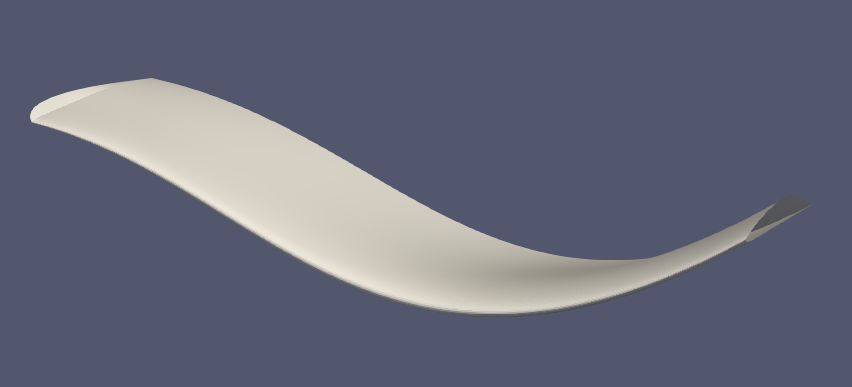
\includegraphics[width = 0.95\textwidth, height = 60mm]{figures/wing_13_iso.png}}
    \caption{Local optima 2}
    \label{local optima 2}
\end{figure}

\begin{figure}[!htbp]
    \centering
    \framebox{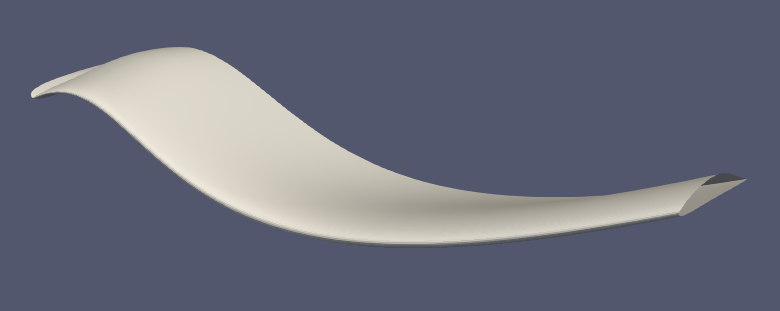
\includegraphics[width = 0.95\textwidth, height = 60mm]{figures/wing_20_iso.png}}
    \caption{Local optima 3}
    \label{local optima 3}
\end{figure}

\begin{figure}
    \centering
    \framebox{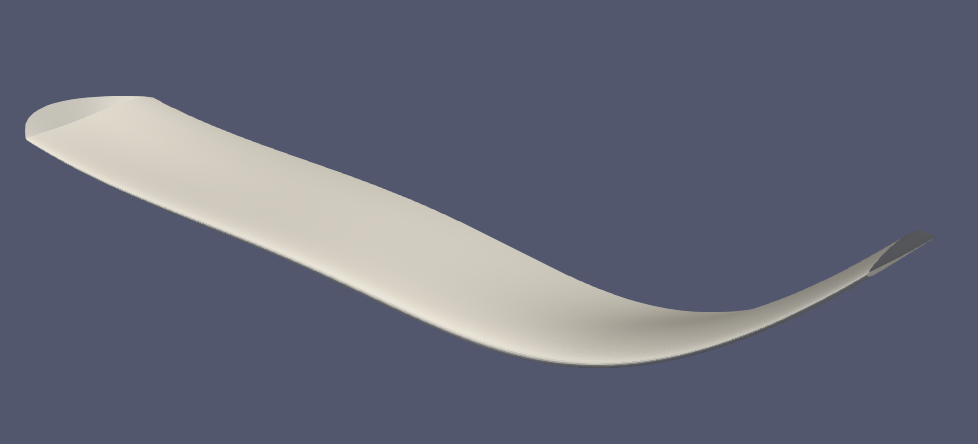
\includegraphics[width = 0.95\textwidth, height = 60mm]{figures/wing_14_iso.png}}
    \caption{Local optima 4}
    \label{local optima 4}
\end{figure}

Assuming that the CFD solution is correct, figure \ref{local optima 2} to \ref{local optima 4} represents the local optima in the increasing order of their objective values. Local optima 2 (figure \ref{local optima 2}) show an anhedral behaviour at the root section and dihedral at the wing tip section. There exists a smooth transition between an anhedral and the dihedral wing sections. Local optima 3 (figure \ref{local optima 3}) contain the waveform at the wing-tip section. Furthermore, a small leading-edge sweepback angle is observed in the root section. Local optima 4 (figure \ref{local optima 4}) reach the upper limit of span (3.3 units). 

The objective function of these optima varies by less than 9\%. As compared to results in Chernukhin \cite{oleg:phd}, the relative difference of objective function is on the higher side. The mesh size that is generated by the glyph script is five times lower. Furthermore, the objective function is found to be ten times higher.

\section{Future work}
This work addresses some of the issues with regards to the implementation of the FFD box, choice of design space, the dimension reduction techniques, winglet creations, and others. There exists some more critical question that needs to be addressed. As mentioned, the glyph script failed to reach the expectation. Further work is necessary to improve the performance of glyph script. Also, the choice of design space needs to be examined.

Further, niching algorithms requires computationally expensive CFD simulation. Reducing the number of CFD runs will significantly reduce the time taken for full optimization. As mentioned by Chernukhin \cite{oleg:phd}, performing the optimization under viscous flowfield will decrease the number of optima. Once all the above objectives are addressed, the work can further extended to viscous flowfield. 
